\section{Setup}
\label{sec:setup}

\begin{figure}[t]
  \centering
  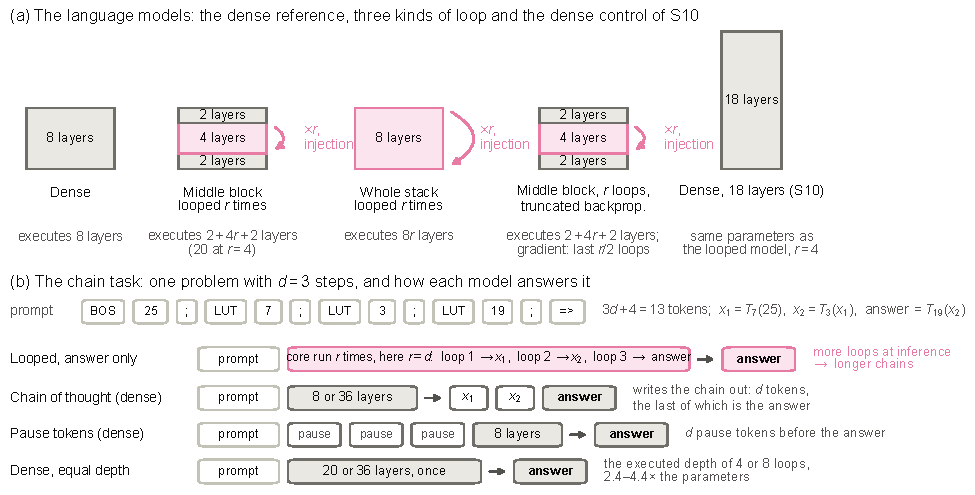
\includegraphics[width=\linewidth]{fig2_schematic}
  \caption{The models and the chain task. \textbf{(a)}~Every language model of the pre-registered grid has eight unique layers. A
  middle-block looped model runs its middle four layers $r$ times; a whole-stack model runs all eight. Each loop starts
  from a linear map of the previous state concatenated with the prelude output (input injection). With truncated
  backpropagation, only the last $r/2$ loops receive gradients. S10 adds dense models with 18 layers and about the looped model's number of parameters (Section~\ref{sec:depth}). \textbf{(b)}~A chain-task problem with $d = 3$ lookups in fixed
  random tables $T_k$ (\texttt{LUT k}: look up table $k$; BOS: the start marker). The looped model answers in one forward pass and computes the chain inside the loop (drawn with
  one loop per step); run for more loops, it solves longer chains. A dense chain-of-thought model writes the $d$ values
  of the chain, the last of which is the answer. A dense model with $d$ pause tokens and a dense model of the looped
  model's executed depth answer in one pass.}
  \label{fig:schematic}
\end{figure}

\subsection{Models}
\label{sec:models}

All language models of the grid (Figure~\ref{fig:schematic}a) are decoder-only transformers with eight unique layers of
width $w$. They use pre-norm RMSNorm, SwiGLU feed-forward blocks (hidden size $\tfrac{8}{3}w$), rotary position
embeddings, attention heads of dimension 64, no biases, untied input and output embeddings, a 16k BPE vocabulary trained
on the training data, and a context of 1024 tokens.

The models differ only in how they run these layers. A \emph{dense} model runs its eight layers once. A
\emph{middle-block} looped model runs the first two layers once (the prelude), the middle four $r$ times (the core, or
looped block) and the last two once (the coda), so it executes $2 + 4r + 2$ layers; a \emph{whole-stack} looped model
runs all eight layers $r$ times.


Each loop starts from a linear map of the previous state concatenated with the prelude output (for the whole stack,
which has no prelude, the embedded input). This input injection, as in Huginn \citep{geiping2025scaling}, has $2w^2$
parameters; the first state is zero. Every residual branch is scaled by $(L/12)^{-1/2}$, a depth rule in which $L = 8$ is the number of unique layers and 12
the reference depth, and by a further $1/r$ inside the core. The scaling is meant to keep the best learning rate
independent of $r$ \citep{wang2026residual}; Appendix~\ref{app:training} checks this. Backpropagation runs through all
loops or, in \emph{truncated} runs, through the last $r/2$ loops only. A model's \emph{executed depth} is the number of
layers it runs: 8 for the dense model and $2 + 4r + 2$ for the middle block. Most text results are for \emph{the 4-loop
model}: the middle block looped 4 times with full backpropagation, which runs 20 layers.

There are five sizes, named by their approximate non-embedding parameters: 10M, 20M, 40M, 80M and 160M, with widths 320
to 1280. Their parameter counts are $N = 15.4$M, 26.8M, 50.1M, 92.7M and 179.6M. $N$ counts the non-embedding parameters and
also the output head \citep{porian2024resolving}, which is large at small widths with a 16k vocabulary (Table~\ref{tab:sizes} in
Appendix~\ref{app:training}).

\subsection{Data, training and the grid}
\label{sec:grid}

Every run, except those of one supplementary experiment that varies the data order (S7), reads a prefix of one
fixed-order stream: files 000--012 of
FineWeb-Edu sample-10BT \citep{penedo2024fineweb}. The stream has 10.4B tokens with our tokeniser and the longest run uses
9.9B, so no run sees a document twice. The main validation set is 50M held-out FineWeb-Edu tokens from file 013. Three
further sets of 20M tokens come from SlimPajama \citep{soboleva2023slimpajama}, FineMath \citep{allal2025smollm2} and
GitHub code (Appendix~\ref{app:training}).

We use AdamW ($\beta = (0.9, 0.95)$, weight decay 0.1, gradient clipping 1.0) with one learning
rate per width, chosen by a sweep on the dense models and used unchanged for the looped models. This rate applies to the
embedding and output layers; the hidden layers use $(8/12)^{-1/2}$ times it, by the same depth rule as the residual
scaling (Appendix~\ref{app:training}). A budget is the number of training tokens per parameter, written $10N$ for ten tokens
per parameter. The schedule is warm-up--stable--decay with cooldown branches \citep{hagele2024scaling}: each run has
one constant-rate trunk, and for each budget a cooldown branches off it at 80\% of the budget and decays the rate
linearly to zero at the budget. Each run therefore gives one result per budget.

Looped runs have budgets of $10N$, $20N$ and $40N$; dense runs $5N$ to $80N$ ($40N$ at 160M). Each looped size
(10M--80M) has ten cells: the middle block with $r = 2$, 4 and 8 and full backpropagation, and with $r = 4$ and 8 and
truncated backpropagation; and the same five for the whole stack. Each size also has one dense model. Every looped cell and dense model has three seeds at
10M--40M and one at 80M, and a 160M dense model serves as a reference: 100 looped and 11 dense runs, 111 in the
pre-registered grid. Seeds change the initialisation,
not the data order.

Extensions of the grid, reported as exploratory, add a 160M 4-loop model and a second 160M dense seed, and continue
10M models to $160N$ and 20M models to $80N$
(Appendix~\ref{app:training} lists the cells and seeds). They also train 20M models with a random loop count, a
regime the pre-registration declared out of scope. Ten supplementary experiments, S1--S10, ran under plans frozen before their runs
(Table~\ref{tab:supp} in Appendix~\ref{app:training}). Everything ran on four RTX 4090 GPUs, about 19 days of wall-clock
time in all.

\subsection{Measurement}
\label{sec:measurement}

Losses are in nats per token on the main validation set. Across initialisation seeds, the loss of the 20M dense model
spans 0.014--0.024 nats at $10N$--$40N$ (0.004--0.008 at 10M and 40M; 0.003--0.07 across the looped cells at 20M).
Pairing runs by seed does not remove this noise. Runs with the same seed and width start from the same weights in the
layers they share and read the same data, yet the gap between the 4-loop model and the dense model of the same seed
varies across seeds by 0.005--0.020 nats at 10M, 0.032--0.045 at 20M and 0.003--0.005 at 40M. A difference of 0.01
nats in one seed is therefore within the noise at 10M--20M and resolvable at 40M. The grid's results at 10M--40M are
means over three seeds.

The pre-registered analysis measures the value of a loop through the effective size of a looped model, $\Neff = \Nonce + r^{\varphi}\Nrec$
\citep{schwethelm2026how}, where $\Nonce$ counts the parameters run once and $\Nrec$ those in the loop. Unlike
\citet{schwethelm2026how}, who count non-embedding parameters only, we include the output head in $\Nonce$, as in $N$.
A dense ``ruler'' $L(N, D) = E + A N^{-\alpha} + B D^{-\beta}$ is fitted to the dense runs
\citep{hoffmann2022training,besiroglu2024chinchilla} with a Huber loss in log space and block-bootstrap intervals
(Appendix~\ref{app:fits}). With the ruler fixed, the primary analysis fits one $\varphi$ for each loop type, that
is, each combination of looped block and backpropagation (the four rows of Table~\ref{tab:prereg}), so that the ruler
evaluated at $\Neff$ matches the looped losses. A joint fit of the ruler and all $\varphi$ is the pre-registered
secondary analysis.

Three further measures need no fitted law. The \emph{gap} is the looped minus the dense loss at equal parameters and
tokens, with the same seed. The \emph{dense size of equal loss}, $\Nstar$, is the size of a dense model that would reach the looped model's
  loss on the same number of training tokens. We read each measured dense size's loss at that token count and
  interpolate $\log N$ linearly in the loss. The \emph{multiplier} $M = \Nstar/N$ says how many dense parameters each
  parameter of the looped model is worth; $M > 1$ means the looped model beats a dense model of its own size. A local
  exponent $\varphi_{\mathrm{loc}}$ is defined by $\Nstar = \Nonce + r^{\varphi_{\mathrm{loc}}}\Nrec$. Finally, the
\emph{equal-compute gap} is the looped loss minus the loss of a dense model of the same size trained with the
  same FLOPs. We convert a looped run's training FLOPs (counted over executed layers, including attention and the output
  head) into the tokens a dense model of the same size could have seen with them. We then read the
  dense loss at that number of tokens off the measured dense curve. Where that point lies beyond the measured curve, two extrapolations bound it (Section~\ref{sec:equalcompute}).

\subsection{Hypotheses and evidence labels}
\label{sec:hypotheses}

The pre-registration was frozen on 2026-09-23, before any training run. It states four hypotheses with decision rules
(Appendix~\ref{app:prereg}):
\begin{itemize}
  \item \textbf{H1}: truncated backpropagation lowers $\varphi$, under both an equal-token and an equal-FLOP accounting.
  \item \textbf{H2}: a looped middle block has a higher $\varphi$ than a looped whole stack.
  \item \textbf{H3}: the gain from extra loops saturates in $r$, so that a geometric form
  $\Neff = \Nonce + \Nrec(1-\rho^r)/(1-\rho)$, with a fitted ratio $\rho$, extrapolates better than $r^{\varphi}$ to a
  held-out size.
  \item \textbf{H4}: the compute-optimal $r$ is small at matched training FLOPs and larger at matched deployment FLOPs.
\end{itemize}
Each result carries one of three labels. \lbl{Pre-registered} results test a hypothesis and decision rule frozen
before training. \lbl{Pre-specified} results were written into a plan frozen before the runs they describe: the
synthetic design (2026-10-09) and the three supplementary plans (2026-10-13, 2026-10-15 and 2026-10-27). These plans
call their experiments exploratory because they lie outside the pre-registration, but their quantities and readings were
fixed before the runs. \lbl{Exploratory} results were chosen after seeing data.
Every departure from a frozen document is dated in the deviation log.
